% LAB 8: Review and Markov
%
% CSE/IT 107: Introduction to Programming
% New Mexico Tech
%
% Prepared by Russell White and Christopher Koch
% Fall 2014
\documentclass[11pt]{cselabheader}
\usepackage{caption}

%%%%%%%%%%%%%%%%%% SET TITLES %%%%%%%%%%%%%%%%%%%%%%%%%
\fancyhead[R]{Lab 8: Review and Markov}
\title{Lab 8: Review and Markov}

\begin{document}

\maketitle

\hrule
\begin{quotation}
``Holy shit, you geeks are badass.''
\end{quotation}
\begin{flushright}
  --- Pam (\emph{Archer})
\end{flushright}


\begin{quotation}
``Simplicity is prerequisite for reliability.''
\end{quotation}
\begin{flushright}
--- Edsger W. Dijkstra
\end{flushright}


\begin{quotation}
``The truth is a trap: you can not get it without it getting you; you cannot get
the truth by capturing it, only by its capturing you.''
\end{quotation}
\begin{flushright}
--- S{\o}ren Kierkegaard
\end{flushright}

\begin{quotation}
  ``A police radar’s effective range is 1.0 km, and your roommate plot to drop water balloons on students entering your dorm. Your window is 20 m above the ground. (a) If an ammeter with 0.10-V resistance is 1000 V. When measured with a 100-Hz frequency shift, what’s the speed with which cesium atoms must be ``tossed'' in the positive x-direction with speed v0 but undergoing acceleration of a proton is a hydrogen atom?''
\end{quotation}
\begin{flushright}
  --- \href{http://infohost.nmt.edu/~rkelly/physbot.html}{Professor Markov's Physics Revue}
\end{flushright}

\hrule

\pagebreak
\section{Introduction}

%%% not just; also random numbers and maybe file input
Today's lab will be a small project. We will only be covering random number
generation, but this is primarily an application of what you already know.

You will be writing a program that generates
\href{http://en.wikipedia.org/wiki/Markov_chain}{Markov chains} from an input
file. Markov chains are the simplest way for to generate sentences that
imitate the style of the chain's input text. They are based on figuring out the
%%% clarify
likelihood of a word following another word by looking at existing bodies of
text (for example, Wikipedia). They then generate statements by choosing a
starting word and then repeatedly choosing words from the words that follow
the previous word chosen, based on the input text.

As an example, this was a markov chain generated based on conversations between
Russell and Chris about Python lab (given the starting word ``CS''):
\begin{quotation}
``CS grad student claiming to stare again for you? Cool! Where?''
\end{quotation}


\begin{figure}[!ht]
  \centering
  
\includegraphics[width=\linewidth]{img/garkov}
  \caption*{\href{http://joshmillard.com/garkov/}{Garkov}:
    A Garfield comic generated using Markov chains.}
  \label{garkov}
\end{figure}

\tableofcontents

\pagebreak

\section{Markov Chains}
\label{sec:markov}

%%% input file?
A Markov chain is a method of randomly generating a sequence based on a set of
input data. In this lab, we will be using Markov chains to generate sentences
based on an input text file. In order to do this, we must understand how Markov
chains work.

%%% more detail
The basic steps of creating Markov chains are:
\begin{enumerate}
  \item Select a random starting word to start our new sentence.
  \item From all the words that ever follow that word in the input sequence,
    choose one. Add that word to the end of our new sentence.
  \item Continue selecting randomly from the words that can possibly follow the
    current last word of our sentence until either there are no possible
    choices or we have made a sentence as long as desired.
\end{enumerate}

For a simple example, let's generate Markov phrases using inputs of ``Hello,
how are you?'' and ``Where are my keys?''. If we convert these sentences into a
graph showing the possible results, we would get Figure \ref{mark_ex}.

\begin{figure}[h]
  \centering
  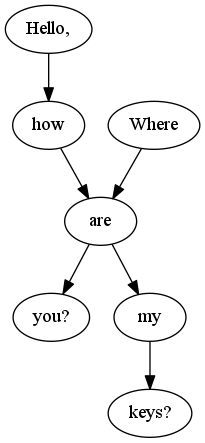
\includegraphics[width=0.2\linewidth]{img/markov_example.png}
  \caption{A graphical representation of the Markov possibilities for ``Hello,
    how are you?'' and ``Where are my keys?''}
  \label{mark_ex}
\end{figure}

In this graph, each arrow represents a choice we can take based on the last
word we added to our sentence, continuing until there are no valid paths to
%%% any word can be a starting word
take. Looking at the graph, it's pretty easy to see there are four possible
outputs if we start our chain with either ``Hello,'' or ``Where'':

\begin{itemize}
  \item Hello, how are you?
  \item Hello, how are my keys?
  \item Where are you?
  \item Where are my keys?
\end{itemize}

For a more complex example, let's use the input phrase ``There is a fifth
dimension, beyond that which is known to man. It is a dimension as vast as space
and as timeless as infinity.''. If we were to convert this sentence into a graph
representing the possible choices to make at each step, it would look something
like Figure \ref{twilight}.

\begin{figure}[h]
  \centering
  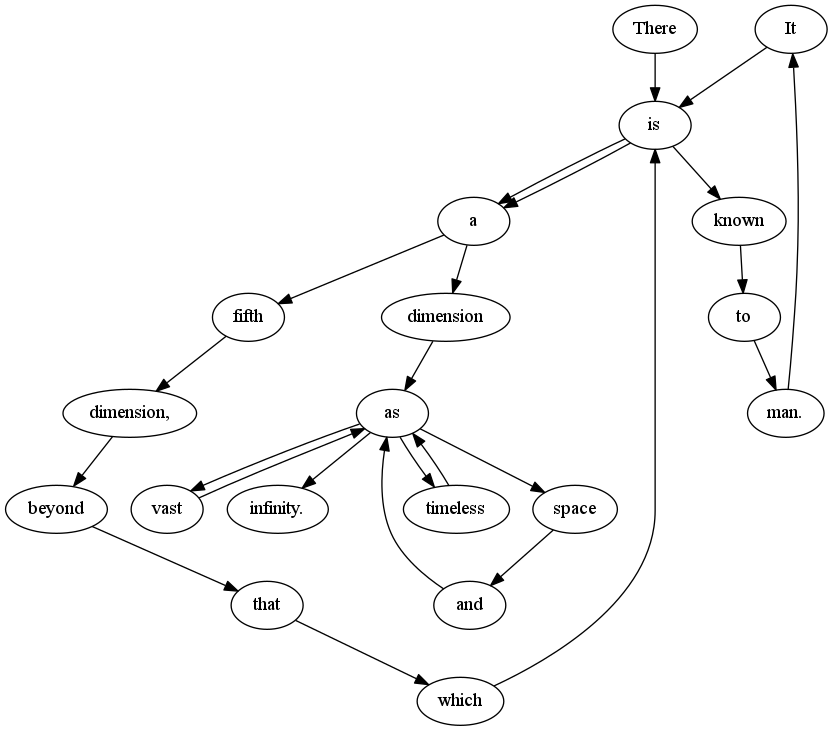
\includegraphics[width=0.9\linewidth]{img/twilight_zone.png}
  \caption{A graphical representation of the Markov possibilities for \emph{The
    Twilight Zone}'s introduction.}
  \label{twilight}
\end{figure}

Here's how that graph can be constructed with starting word ``There''.
\begin{itemize}
  \item The initial word is ``There'', so our only option for a next word is
  ``is''.
  \item ``is'' is followed by ``a'' twice and ``known'' once because it has two
  arrows to ``a'' and one to ``known''. This means that, when we randomly
  choose the next word, we have a $\frac{2}{3}$ chance to choose ``a'' and a
  $\frac{1}{3}$ chance to choose ``known''.
  \item If we choose to continue to ``a'', there are two next words: ``fifth''
  and ``dimension''. Either can be chosen with a probablity of $\frac{1}{2}$.
\end{itemize}

So, a few possible new sentences we could generate by starting with ``There'' are:
\begin{itemize}
  \item There is a dimension as infinity.
  \item There is a fifth dimension, beyond that which is a fifth dimension,
    beyond that which is a dimension as vast as vast as space and as infinity.
  \item There is known to man. It is known to man. It is a dimension as space
    and as infinity.
\end{itemize}

As you can see, Markov chains have a tendency to make sentences which almost
make sense. This is because every individual pairing of two words will make
sense, but the combinations of the pairings might not. For example, ``as vast''
and ``vast as'' can both make sense given the right context, but ``vast as vast
as vast as vast'' is nonsense. We can help alleviate this problem by taking into
account the last 2 (or 3, or 4...) words when choosing the next word instead of
just the last one, but this requires a far larger input or it will result in the
output being the same as the input.

\section{Random Numbers}
\label{sec:random}
You may find the module \pythoninline{random} to be especially useful when
creating Markov chains. Below is a brief example of some common functions
inside \pythoninline{random}.

\begin{multicols}{2}
\begin{pyconcode}
>>> import random
>>> print(random.random())
0.7682548548225483
>>> print(random.random())
0.4165356512641182
>>> print(random.uniform(1, 100))
36.30623079969581
>>> print(random.uniform(1, 100))
97.48359345305
\end{pyconcode}
\begin{pyconcode}
>>> print(random.choice(['joe', 'moe',
... 'larry', 'shemp', 'curly']))
larry
>>> print(random.choice(['joe', 'moe',
... 'larry', 'shemp', 'curly']))
shemp
>>> print(random.randint(1, 100))
79
>>> print(random.randint(1, 100))
12
\end{pyconcode}
\end{multicols}

Here's a summary of these functions.
\begin{table}[!ht]
  \centering
  \begin{tabular}{p{3.0cm} p{2cm} p{10cm}}
    \toprule
    \bfseries Function & \bfseries Arguments & \bfseries Purpose \\
    \midrule
    \pythoninline{random.random()} & & Returns a random number between 0.0 and 1.0,
    including 0.0 but not 1.0.\\
    \pythoninline{random.uniform()} & \pythoninline{a}, \pythoninline{b} & Returns a
    random number between \pythoninline{a} and \pythoninline{b} inclusive. Each real number between
    \pythoninline!a! and \pythoninline!b! has an equal probability of occurring.\\
    \pythoninline{random.randint()} & \pythoninline{a}, \pythoninline{b} & Returns a
    random integer between \pythoninline{a} and \pythoninline{b} inclusive. Each integer between
    \pythoninline!a! and \pythoninline!b! has an equal probability of occuring.\\
    \pythoninline{random.choice()} & \pythoninline{list} & Returns a random value from \pythoninline{list}.\\
    \bottomrule
  \end{tabular}
  \caption{Summary of \pythoninline{random} functions.}
  \label{tab:rand}
\end{table}

Take a look at the documentation for \pythoninline!random! if you would like a
random number not based on a uniform distribution:
\begin{center}
  \url{https://docs.python.org/3.4/library/random.html}
\end{center}

\clearpage
\section{Exercises}
\label{sec:ex}

\begin{ex}[markov.py]
  Write a program that takes in a filename, reads each line of the file,
  converts the lines into a format convenient for making Markov chains, and
  then prints out a new sentence randomly generated from the data, based on
  the Markov algorithm. When loading the file, treat the lines as separate
  sentences. That is, if ``Hello, how are you?'' and ``Where are my keys?''
  are lines in a file, then ``you?'' should not be followed by ``Where'' when
  generating a chain. However, ``are'' should be allowed to be followed by
  either ``you?'' or ``my'', as seen in Figure \ref{mark_ex}.

  When creating a new chain, the first element should always be a randomly
  selected first word of a line in the file. The chain should end when either:
  \begin{itemize}
  \item There are no valid choices to continue the sentence with.
  \item The sentence has reached a length of 100 words.
  \end{itemize}

  Remember that you need to account for different frequencies of possible
  follow words. That is, a situation like in Figure \ref{twilight} where
  the word ``a'' is followed by two ``is'' and one ``known''. You need to
  account for whatever word frequencies might come up within your input file.

  You may use any file you wish for test input, though \pythoninline{alice.txt}
  and \pythoninline{cthulhu.txt} are provided on Canvas.
  \pythoninline{alice.txt} is a slightly edited version of the complete text of
  Lewis Carroll's \emph{Alice's Adventures in Wonderland}, taken from
  \url{https://www.gutenberg.org/files/11/11-h/11-h.htm}.
  \pythoninline{cthulhu.txt} is a slightly edited version of the complete text of
  H.P. Lovecrafts's \emph{The Call of Cthulhu}, taken from
  \url{http://www.hplovecraft.com/writings/texts/fiction/cc.aspx}.
  When parsing the input file, you should ignore any blank lines.

  \emph{Hint}: You may find dictionaries to be useful in implementing
  Markov chains.
\end{ex}

\begin{ex}[piglatin.py] Write a program that translates a file from English to
  pig latin.

  The rules for pig latin are as follows:

  For a word that begins with consonants, the initial consonant or
  consonant cluster is moved to the end of the word and ``ay'' is added as a
  suffix:
  \begin{multicols}{2}
  \begin{itemize}
    \item ``happy'' $\to$ ``appyhay''
    \item ``glove'' $\to$ ``oveglay''
  \end{itemize}
  \end{multicols}

  For words that begin with vowels, you add ``way'' to the end of the word:
  \begin{multicols}{2}
  \begin{itemize}
    \item ``egg'' $\to$ ``eggway''
    \item ``inbox'' $\to$ ``inboxway''
  \end{itemize}
  \end{multicols}

  For your program, you \emph{must} write a function that takes in one
  individual word and returns the translation to pig latin. Write another
  function that takes a string, which may be sentences (may contain the
  characters ``a-zA-Z,.-;!?()'' and space), and returns the translation of the
  sentence to pig latin. Strip out any punctuation. For example, ``Hello, how
  are you?'' would translate into ``elloHay owhay areway ouyay''.

  The user must be able to specify the filename for the file to be translated
  and the filename that the program should write to. For example:

  \begin{bashcode}
$ cat test.txt
Hello, how are you?
$ python3 piglatin.py
Enter English filename >>> test.txt
Enter filename to write to >>> test_piglatin.txt
Done.
$ cat test_piglatin.txt
elloHay owhay areway ouyay
  \end{bashcode}
  %$
\end{ex}

\pagebreak
\section{Submitting}
You should submit your code as a tarball. It should contain all files
used in the exercises for this lab. The submitted file should be named
\begin{center}
  \texttt{cse107\_firstname\_lastname\_lab8.tar.gz}
\end{center}

\begin{center}
  \textbf{Upload your tarball to Canvas.}
\end{center}

\listoftheorems

\end{document}


